\chapter{Measurements}

In this chapter, based on the results of the tests presented in the previous chapter, I will try to answer several questions:
\begin{enumerate}
  \item What is the influence of each storage driver on the performance, which one is the best for us?
  \item What is the influence of each container runtime on the performance, which one is the best for us?
  \item What is the influence of each container manager on the performance, which one is the best for us?
  \item What is the influence of each base image on the performance, which one is the best for us?
  \item Does the a rootless container have any performance drawback over a rootfull one?
\end{enumerate}

Based on that, I will try to compose the best solution that should be used in the case of INGInious.

\section{Variabilities influence}

\subsection{Storage driver}
In order to determine the influence of the choice of one storage driver over another, we will concentrate over the results of some of them to the different I/O tests: Large amount of file read and write, and Big file read and write.
We won't be comparing each possible configuration here, I have selected the 16 of them, which are representative enough of the others.  

\clearpage
\subsubsection{Default Docker's case}
We will first start by comparing the six storage drivers proposed by Docker, using as common configuration:

\begin{tabular}{rl}
   \textbf{Container manager} & Docker \\
   \textbf{Container runtime} & runc \\
   \textbf{Base image} & Alpine \\
   \textbf{Control group} & v1 \\
   \textbf{Rootless} & No 
\end{tabular}

This configuration shows similar results as if we changed runc for crun or if we changed Docker for Podman.  The values vary, but the storage driver behave the same way, relatively to one another.


\begin{figure}[h!]
    \begin{subfigure}{.5\textwidth}
      \centering
      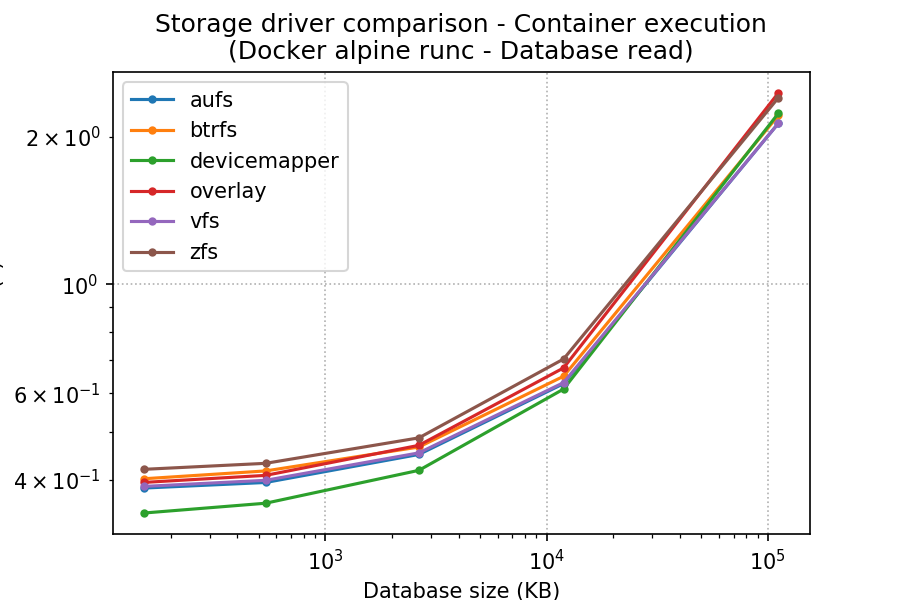
\includegraphics[width=\linewidth]{images/storage-driver/storage-driver-execution-Docker-alpine-runc---Database-read.png}
      \caption{Execution time of containers used for database reading performance test.}
      \label{fig:storage-driver:runc:db-read-exec}
    \end{subfigure}
    \begin{subfigure}{.5\textwidth}
      \centering
      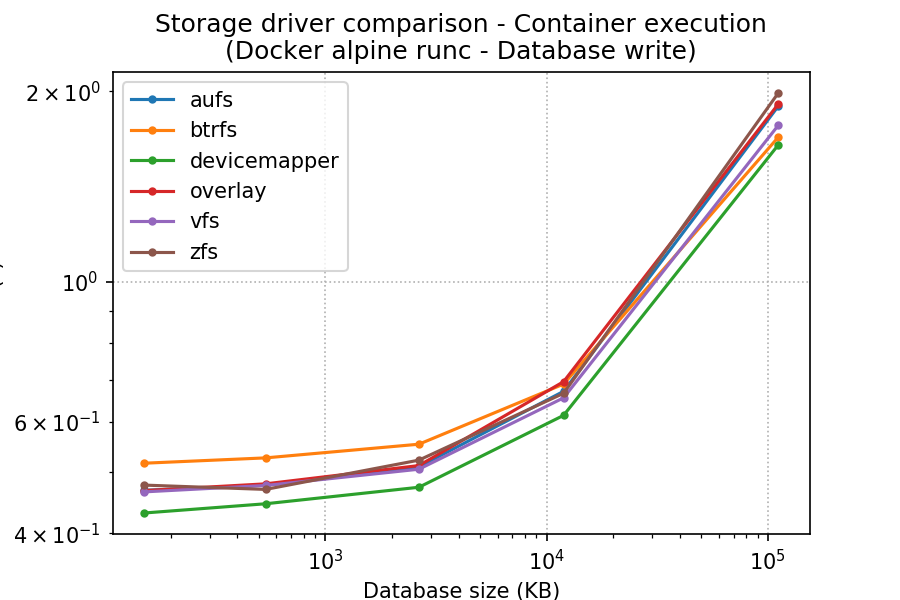
\includegraphics[width=\linewidth]{images/storage-driver/storage-driver-execution-Docker-alpine-runc---Database-write.png}
      \caption{Execution time of containers used for database reading performance test.}
      \label{fig:storage-driver:runc:db-write-exec}
    \end{subfigure}
    
    \begin{subfigure}{.5\textwidth}
      \centering
      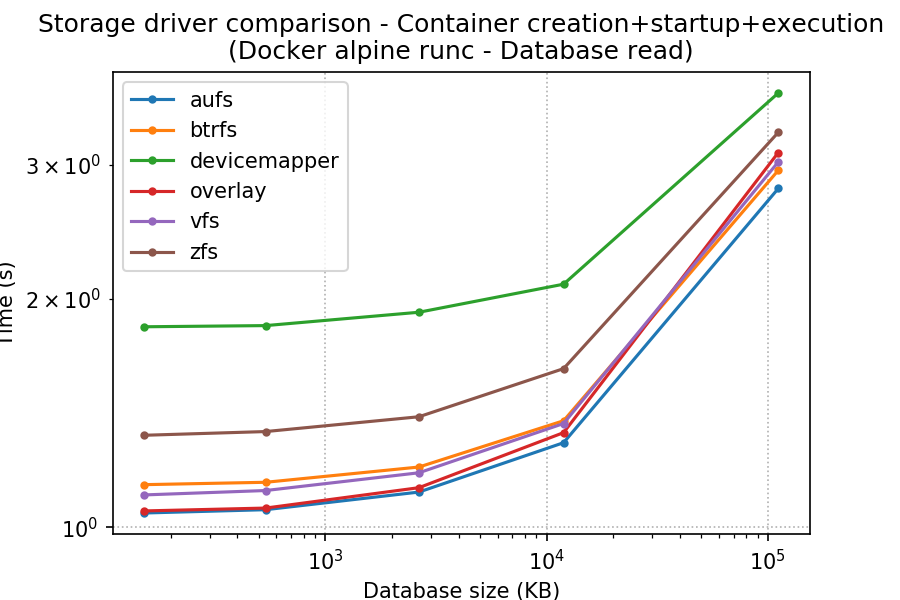
\includegraphics[width=\linewidth]{images/storage-driver/storage-driver-full-Docker-alpine-runc---Database-read.png}
      \caption{Creation, startup and execution time of containers used for database reading performance test.}
      \label{fig:storage-driver:runc:db-read-full}
    \end{subfigure}
    \begin{subfigure}{.5\textwidth}
      \centering
      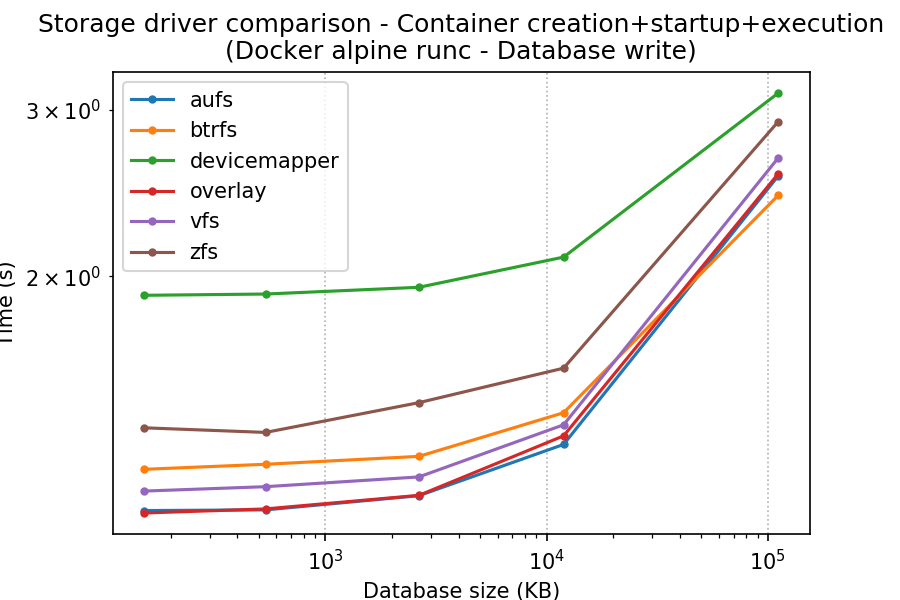
\includegraphics[width=\linewidth]{images/storage-driver/storage-driver-full-Docker-alpine-runc---Database-write.png}
      \caption{Creation, startup and execution time of containers used for database writing performance test.}
      \label{fig:storage-driver:runc:db-write-full}
    \end{subfigure}
    
    \caption{Database read and write tests for containers launched with Docker and runc, based on an Alpine image}
\end{figure}

\begin{figure}[!h]
    \begin{subfigure}{.5\textwidth}
      \centering
      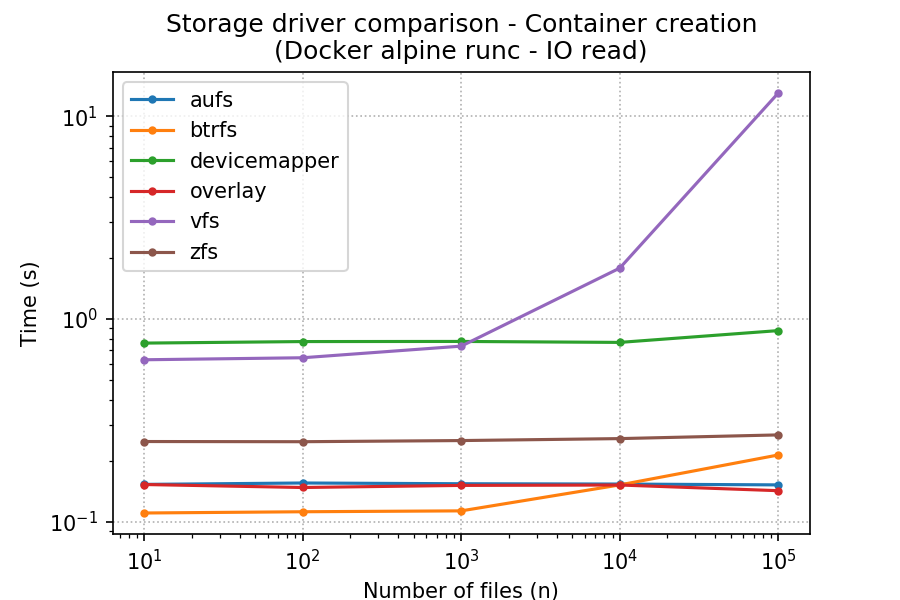
\includegraphics[width=\linewidth]{images/storage-driver/storage-driver-creation-Docker-alpine-runc---IO-read.png}
      \caption{Average creation time of containers depending on the number of files in one folder.}
      \label{fig:storage-driver:runc:io-read-create}
    \end{subfigure}
    \begin{subfigure}{.5\textwidth}
      \centering
      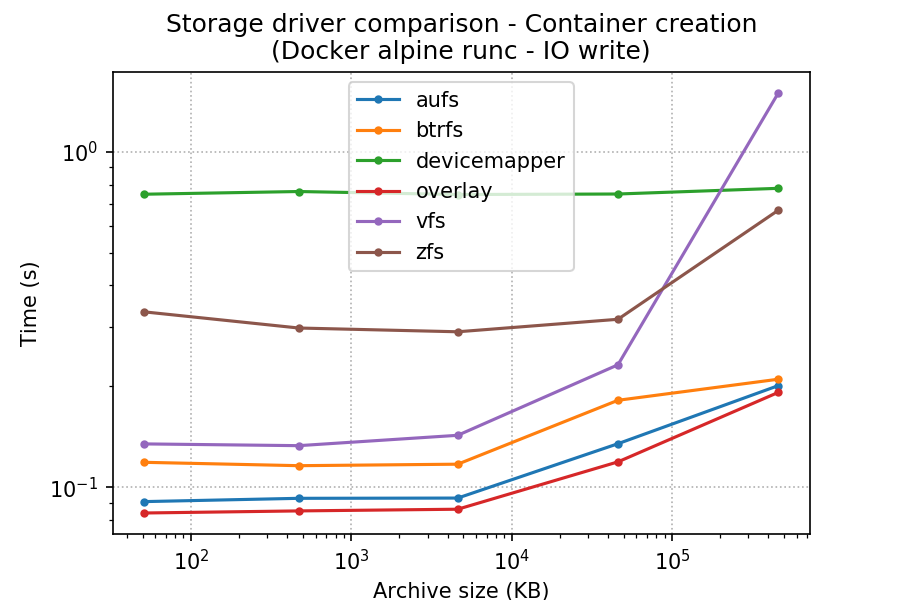
\includegraphics[width=\linewidth]{images/storage-driver/storage-driver-creation-Docker-alpine-runc---IO-write.png}
      \caption{Average creation time of containers depending on the size of the archive containing all the files.}
      \label{fig:storage-driver:runc:io-write-create}
    \end{subfigure}
    
    % \begin{subfigure}{.5\textwidth}
    %   \centering
    %   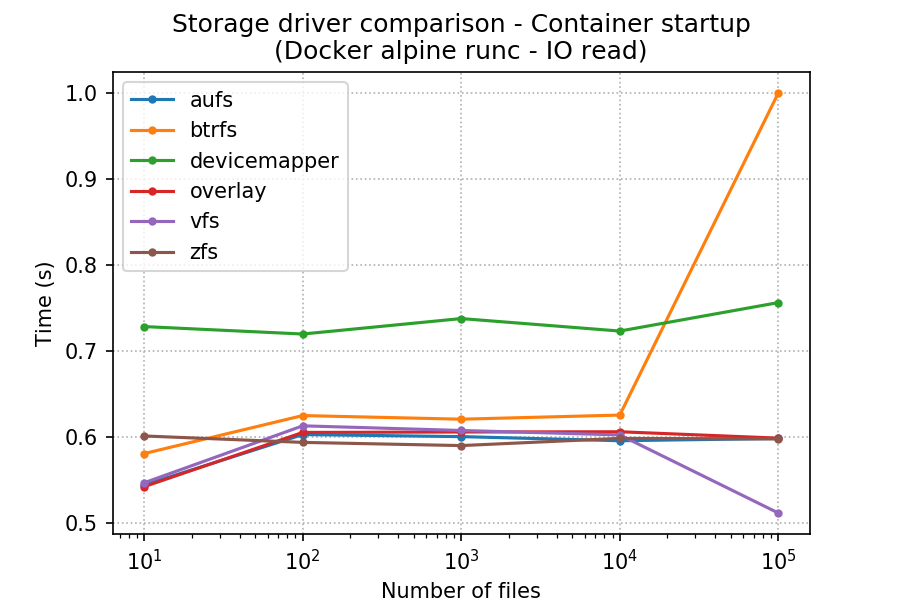
\includegraphics[width=\linewidth]{images/storage-driver/storage-driver-startup-Docker-alpine-runc---IO-read.png}
    %   \caption{Starting time of containers used for IO reading performance test.}
    %   \label{fig:storage-driver:runc:io-read-start}
    % \end{subfigure}
    % \begin{subfigure}{.5\textwidth}
    %   \centering
    %   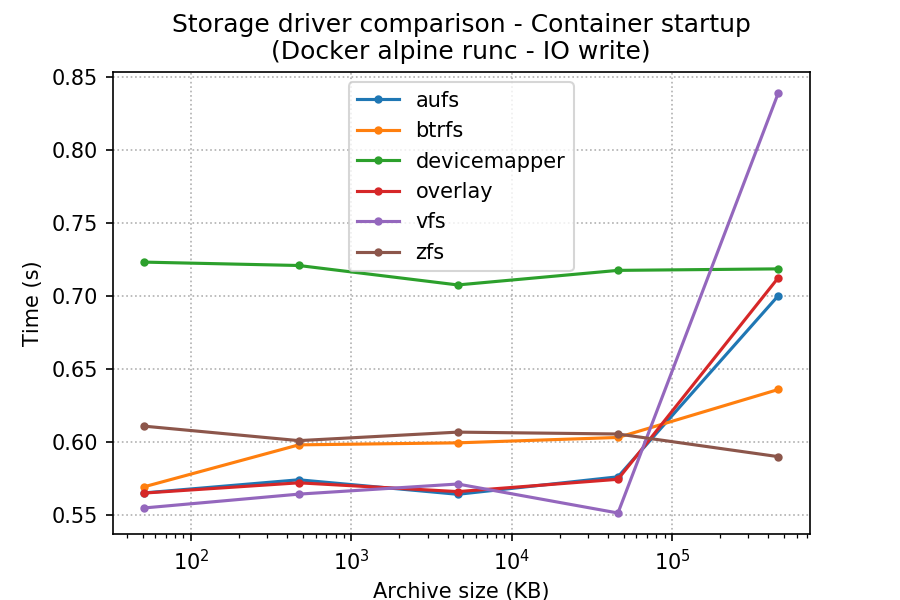
\includegraphics[width=\linewidth]{images/storage-driver/storage-driver-startup-Docker-alpine-runc---IO-write.png}
    %   \caption{Starting time of containers used for IO writing performance test.}
    %   \label{fig:storage-driver:runc:io-write-start}
    % \end{subfigure}
    
    \begin{subfigure}{.5\textwidth}
      \centering
      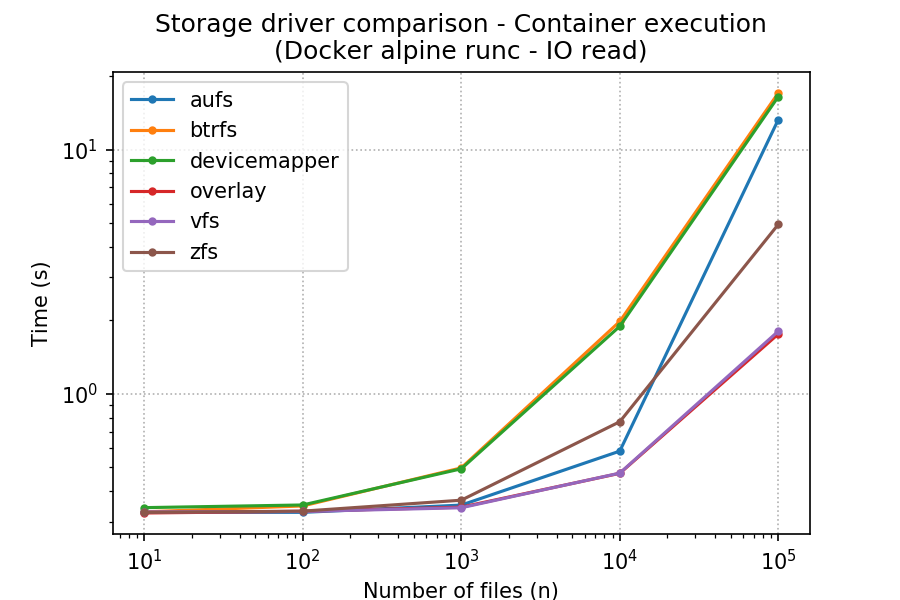
\includegraphics[width=\linewidth]{images/storage-driver/storage-driver-execution-Docker-alpine-runc---IO-read.png}
      \caption{Average total reading time for n files.}
      \label{fig:storage-driver:runc:io-read-exec}
    \end{subfigure}
    \begin{subfigure}{.5\textwidth}
      \centering
      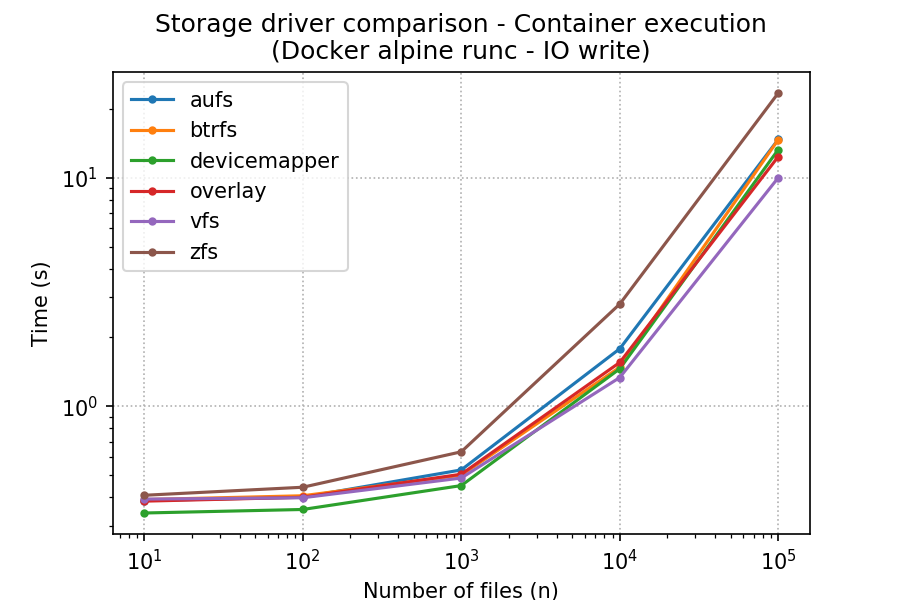
\includegraphics[width=\linewidth]{images/storage-driver/storage-driver-execution-Docker-alpine-runc---IO-write.png}
      \caption{Average extracting time of n files from one (non-compressed) archive.}
      \label{fig:storage-driver:runc:io-write-exec}
    \end{subfigure}
    
    \begin{subfigure}{.5\textwidth}
      \centering
      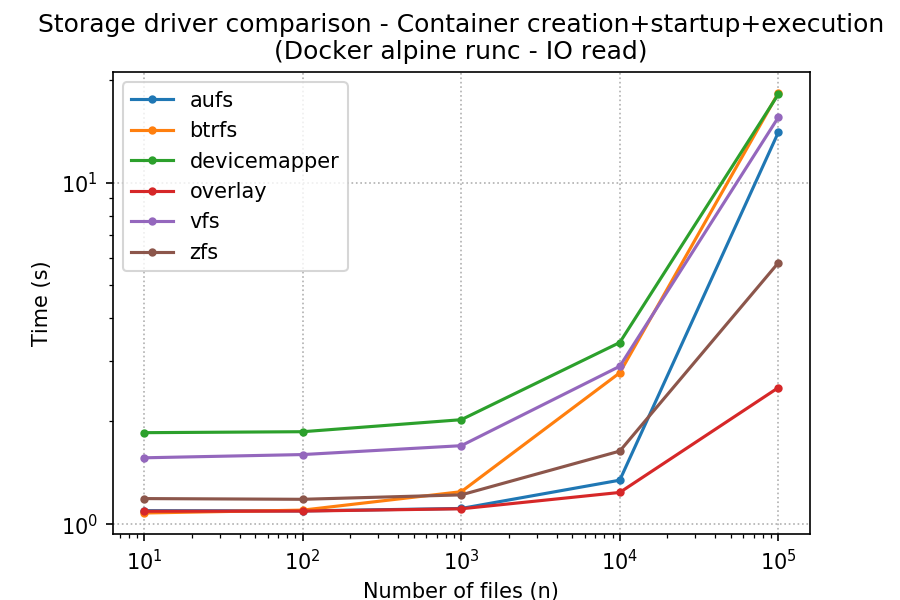
\includegraphics[width=\linewidth]{images/storage-driver/storage-driver-full-Docker-alpine-runc---IO-read.png}
      \caption{Average creation, startup and execution time of containers used for IO reading performance test.}
      \label{fig:storage-driver:runc:io-read-full}
    \end{subfigure}
    \begin{subfigure}{.5\textwidth}
      \centering
      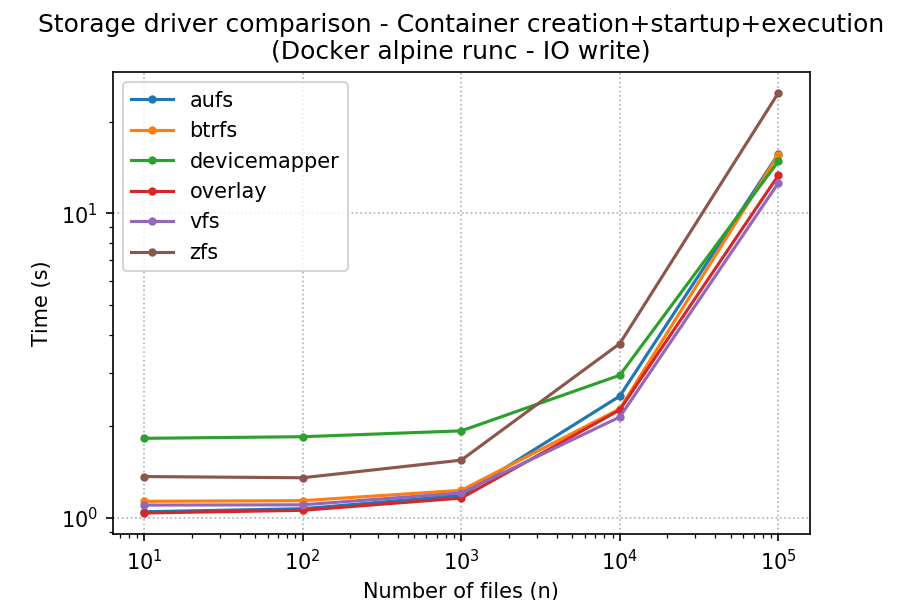
\includegraphics[width=\linewidth]{images/storage-driver/storage-driver-full-Docker-alpine-runc---IO-write.png}
      \caption{Average creation, startup and execution time of containers used for IO reading performance test.}
      \label{fig:storage-driver:runc:io-write-full}
    \end{subfigure}
    
    \caption{IO read and write tests for containers launched with Docker and runc, based on an Alpine image}
\end{figure}

On those figures we can observe the following things:
\begin{enumerate}
  \item As vfs as no copy on write mechanism, it has to copy all the data editable in the container for each container creation.  This gives it a drawback over the other solutions with copy on write capabilities, and it get worse as the size of the container grows.  We can see that on both Figure \ref{fig:storage-driver:runc:io-read-create} and Figure \ref{fig:storage-driver:io-write-create}.
  \item Overlayfs and AUFS are both union filesystems, and their corresponding storage driver perform similarily in most cases.  On Figure \ref{fig:storage-driver:runc:io-read-exec} and Figure \ref{fig:storage-driver:runc:io-write-exec} we can see that this changes, aufs is far behind overlay.  This is because of one significant difference in their implementation; when a file is open with Overlayfs, all the following actions performed on it (read/write) will be directly transfered to the underlying filesystem, overlay has no hand on it.  This is not the case with AUFS, and it is paid heavily when a lot of I/O has to be done.
  \item As vfs as already copied all files on container creation, it is unbeatable for file creation (Figure \ref{fig:storage-driver:runc:io-write-exec}).  The next faster solution is overlay, which even meet vfs performance when it comes to read small files (Figure \ref{fig:storage-driver:runc:io-read-exec}).  This makes overlay the best solution for reading and creating a lot of files, as it has no creation cost, and its file-based copy on write mechanism is apparently the most efficient for those cases.
  \item Devicemapper, btrfs and zfs have block-based copy on write, and in the case of devicemapper and btrfs it gives a great advantage when applying modification to big files.  Indeed with such strategy only the blocks that are modified needs to be copied, while other file-based copy-on-write mechanism will have to copy the whole file.  We can see on Figure \ref{fig:storage-driver:runc:db-write-exec} that they even manage to beat vfs.  Btrfs should be chosen over devicemapper though, as we can see in Figure \ref{fig:storage-driver:runc:db-write-full}, this is because devicemapper containers have a greater creation and starting cost.
\end{enumerate}

% \paragraph{}\textbf{In really short, what storage driver is the more performant?}
% Overlay it the best solution for most scenarios.  For the specific case of big file modification, block-based copy-on-write mechanism are better though, in this case choose btrfs over devicemapper (not supported anymore by Docker since v19.03, and higher container creation cost).


\clearpage
\subsubsection{Kata-container's case}
Those same storage drivers (same implementation) behave very differently when using virtualization-based containers, with Kata-container.  The common configuration will now be:

\begin{tabular}{rl}
   \textbf{Container manager} & Docker \\
   \textbf{Container runtime} & kata-runtime \\
   \textbf{Base image} & Alpine \\
   \textbf{Control group} & v1 \\
   \textbf{Rootless} & No 
\end{tabular}

The behaviour of Kata-container using qemu with devicemapper storage driver correspond to the behaviour of this same driver but with Kata-container using Firecracker as hypervisor.

\begin{figure}[h!]
    \begin{subfigure}{.5\textwidth}
      \centering
      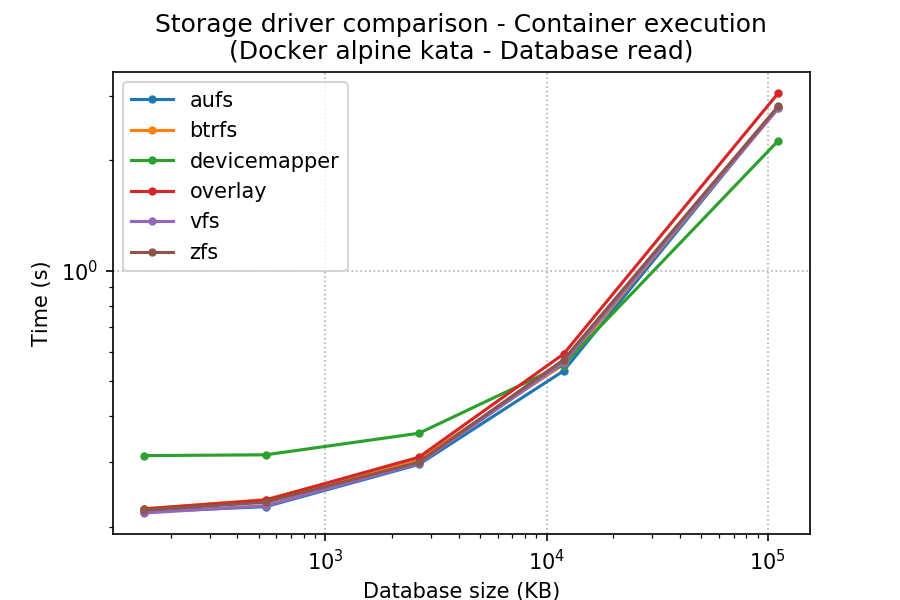
\includegraphics[width=\linewidth]{images/storage-driver/storage-driver-execution-Docker-alpine-kata---Database-read.png}
      \caption{Execution time of containers used for database reading performance test.}
      \label{fig:storage-driver:kata:db-read-exec}
    \end{subfigure}
    \begin{subfigure}{.5\textwidth}
      \centering
      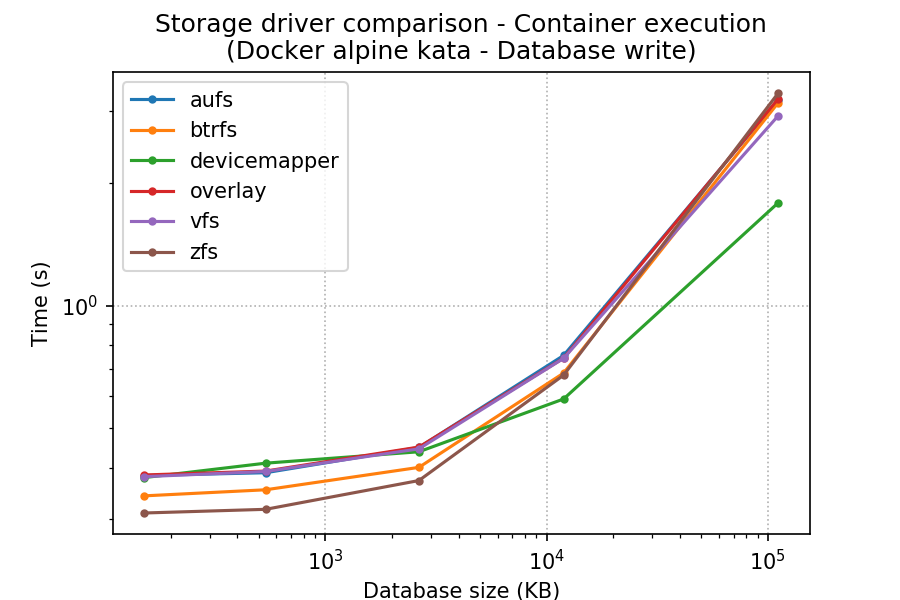
\includegraphics[width=\linewidth]{images/storage-driver/storage-driver-execution-Docker-alpine-kata---Database-write.png}
      \caption{Execution time of containers used for database reading performance test.}
      \label{fig:storage-driver:kata:db-write-exec}
    \end{subfigure}
    
    \begin{subfigure}{.5\textwidth}
      \centering
      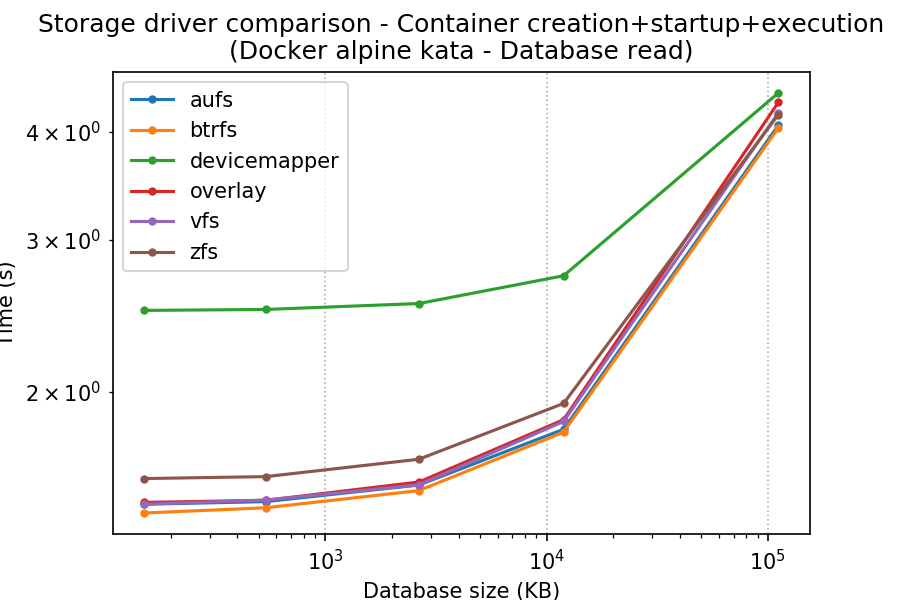
\includegraphics[width=\linewidth]{images/storage-driver/storage-driver-full-Docker-alpine-kata---Database-read.png}
      \caption{Creation, startup and execution time of containers used for database reading performance test.}
      \label{fig:storage-driver:kata:db-read-full}
    \end{subfigure}
    \begin{subfigure}{.5\textwidth}
      \centering
      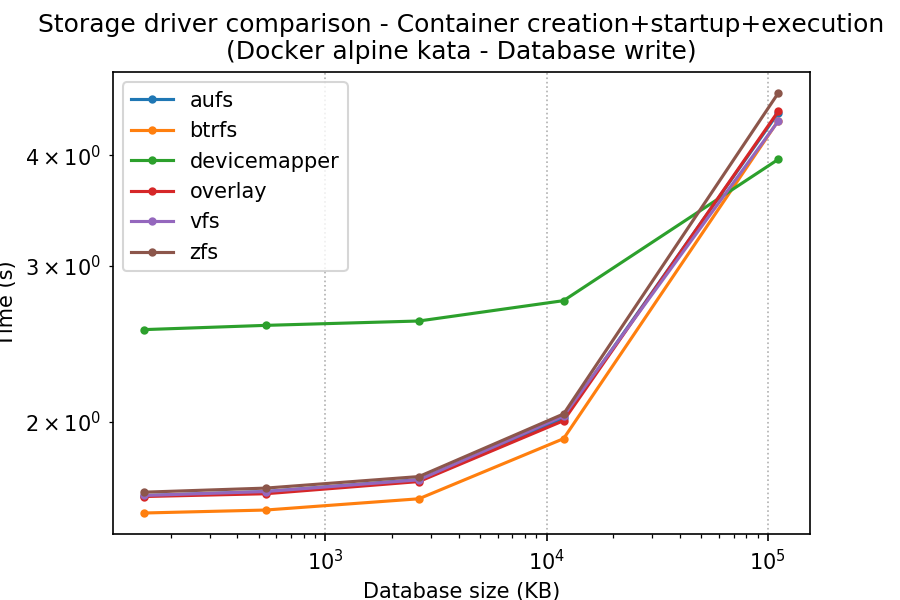
\includegraphics[width=\linewidth]{images/storage-driver/storage-driver-full-Docker-alpine-kata---Database-write.png}
      \caption{Creation, startup and execution time of containers used for database writing performance test.}
      \label{fig:storage-driver:kata:db-write-full}
    \end{subfigure}
    
    \caption{Database read and write tests for containers launched with Docker and Kata-Container (qemu), based on an Alpine image}
    \label{fig:storage-driver:kata:db}
\end{figure}

\begin{figure}[!h]
    
    \begin{subfigure}{.5\textwidth}
      \centering
      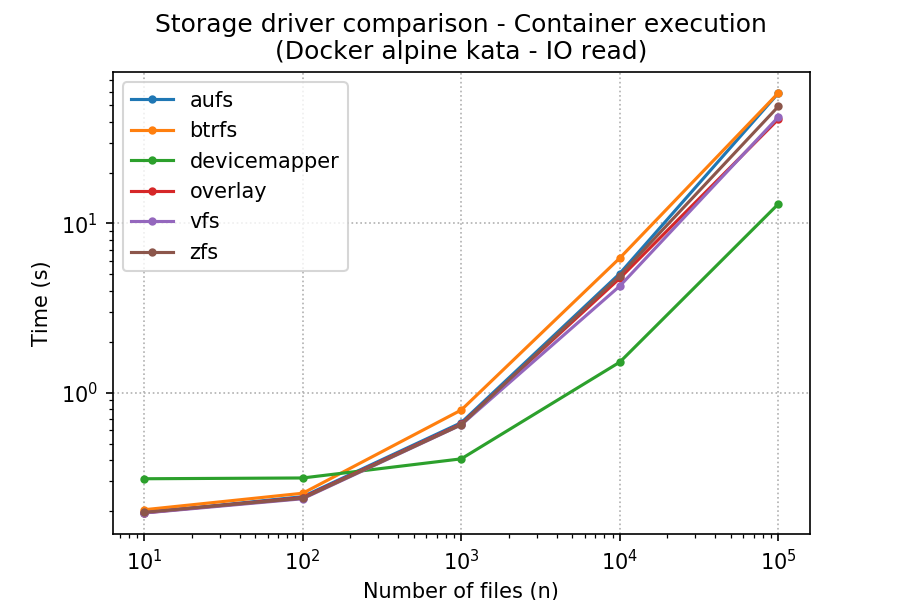
\includegraphics[width=\linewidth]{images/storage-driver/storage-driver-execution-Docker-alpine-kata---IO-read.png}
      \caption{Average total reading time for n files.}
      \label{fig:storage-driver:kata:io-read-exec}
    \end{subfigure}
    \begin{subfigure}{.5\textwidth}
      \centering
      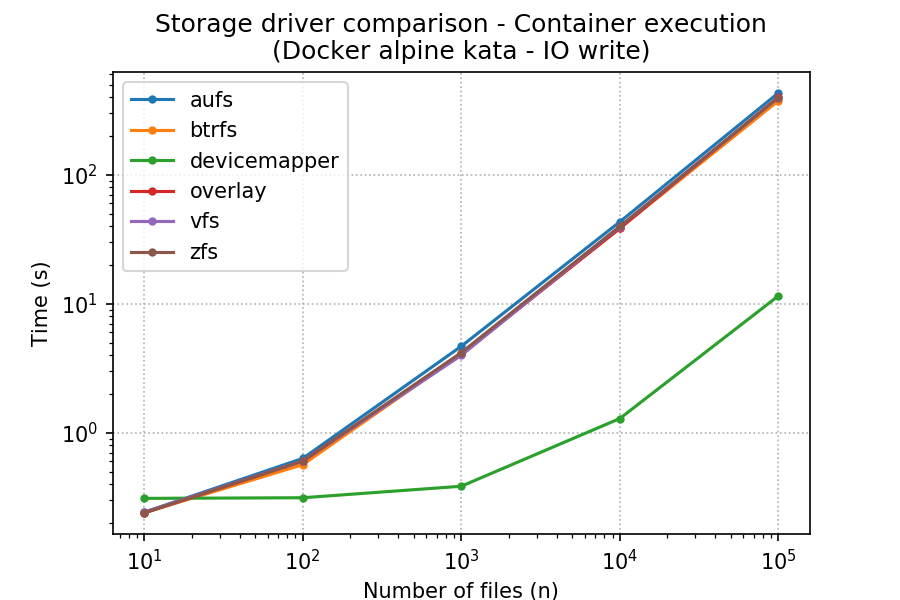
\includegraphics[width=\linewidth]{images/storage-driver/storage-driver-execution-Docker-alpine-kata---IO-write.png}
      \caption{Average extracting time of n files from one (non-compressed) archive.}
      \label{fig:storage-driver:kata:io-write-exec}
    \end{subfigure}
    
    \begin{subfigure}{.5\textwidth}
      \centering
      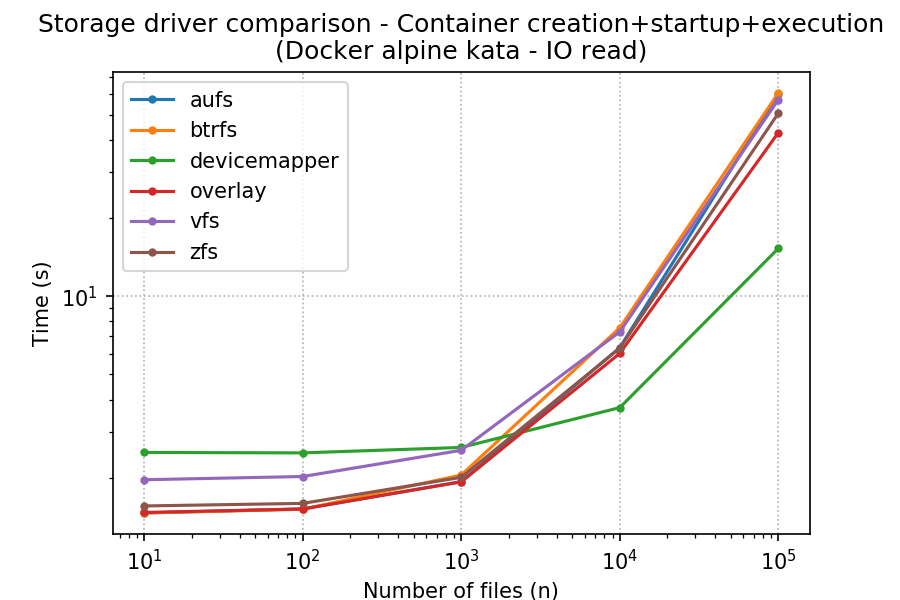
\includegraphics[width=\linewidth]{images/storage-driver/storage-driver-full-Docker-alpine-kata---IO-read.png}
      \caption{Average creation, startup and execution time of containers used for IO reading performance test.}
      \label{fig:storage-driver:kata:io-read-full}
    \end{subfigure}
    \begin{subfigure}{.5\textwidth}
      \centering
      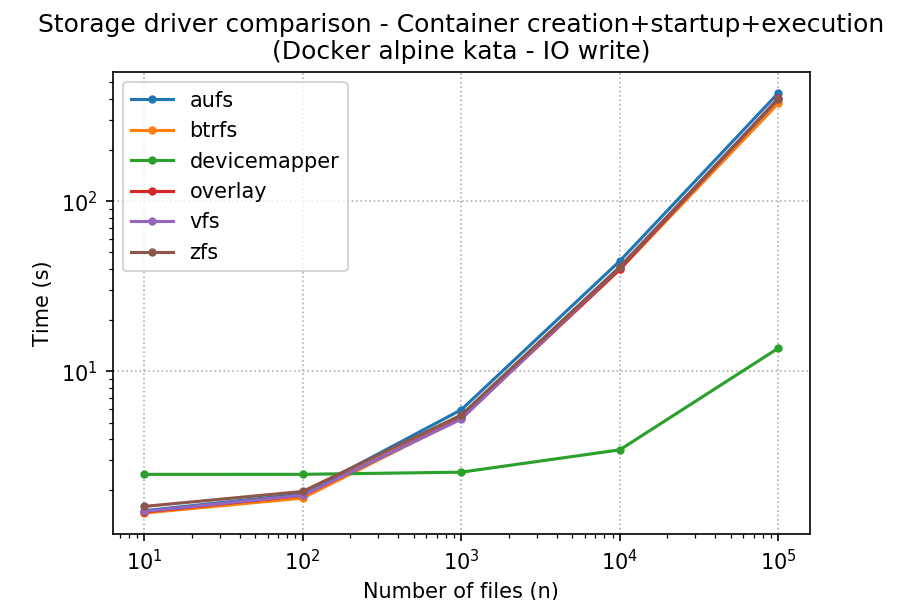
\includegraphics[width=\linewidth]{images/storage-driver/storage-driver-full-Docker-alpine-kata---IO-write.png}
      \caption{Average creation, startup and execution time of containers used for IO reading performance test.}
      \label{fig:storage-driver:kata:io-write-full}
    \end{subfigure}
    
    \caption{IO read and write tests for containers launched with Docker and Kata-Container (qemu), based on an Alpine image}
\end{figure}

\paragraph{}The creation of containers doesn't change that much with kata-container, neither does the startup, everything is just a little bit slower.  For the execution though, thinks get interesting.  Passed a certain point, devicemapper appear to be the only viable solution, and that turning point arrives quite quickly.  As you can see on Figure \ref{fig:storage-driver:kata:io-read-exec} and Figure \ref{fig:storage-driver:kata:io-write-exec}, all other storage drivers follow about the same curve.  It seems that the virtual block devices of devicemapper go well with virtualized solutions.  It kind of makes sense, but unfortunetly I can not explain it.  We can observe this same thing with the database tests (Figure \ref{fig:storage-driver:kata:db}), but it is less obvious than with the other ones.

\clearpage
\subsubsection{LXD's case}
Here the implementation of the storage drivers is different, and less of them are available.  The common configuration will be:

\begin{tabular}{rl}
   \textbf{Container manager} & LXD \\
   \textbf{Container runtime} & LXC \\
   \textbf{Base image} & Alpine \\
   \textbf{Control group} & v1 \\
   \textbf{Rootless} & No 
\end{tabular}

\begin{figure}[h!]
    \begin{subfigure}{.5\textwidth}
      \centering
      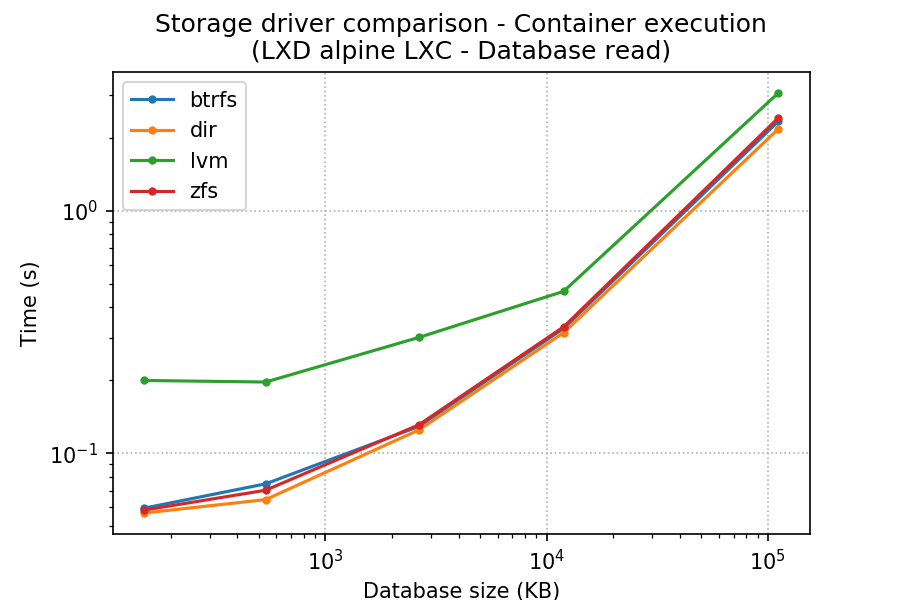
\includegraphics[width=\linewidth]{images/storage-driver/storage-driver-execution-LXD-alpine-LXC---Database-read.png}
      \caption{Execution time of containers used for database reading performance test.}
      \label{fig:storage-driver:lxc:db-read-exec}
    \end{subfigure}
    \begin{subfigure}{.5\textwidth}
      \centering
      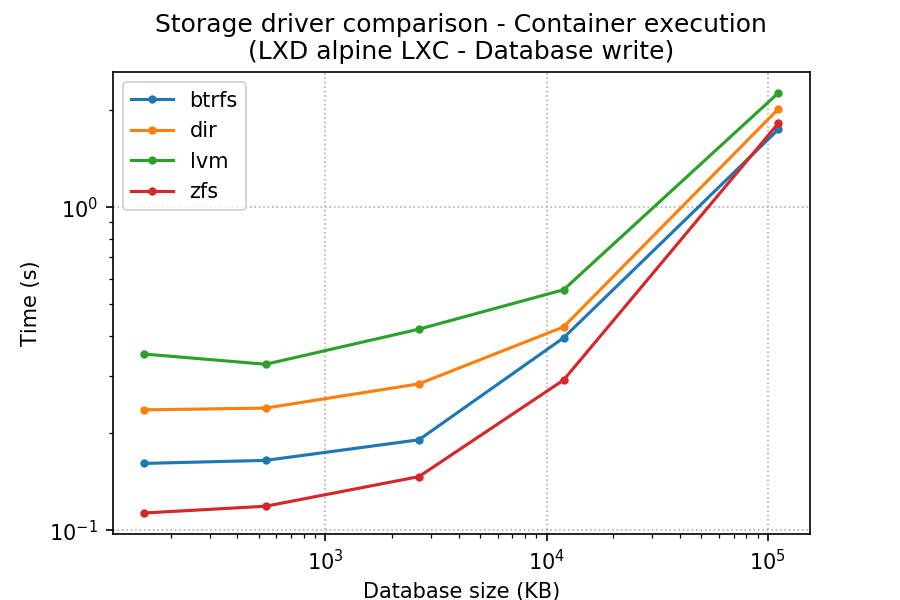
\includegraphics[width=\linewidth]{images/storage-driver/storage-driver-execution-LXD-alpine-LXC---Database-write.png}
      \caption{Execution time of containers used for database reading performance test.}
      \label{fig:storage-driver:lxc:db-write-exec}
    \end{subfigure}
    
    \begin{subfigure}{.5\textwidth}
      \centering
      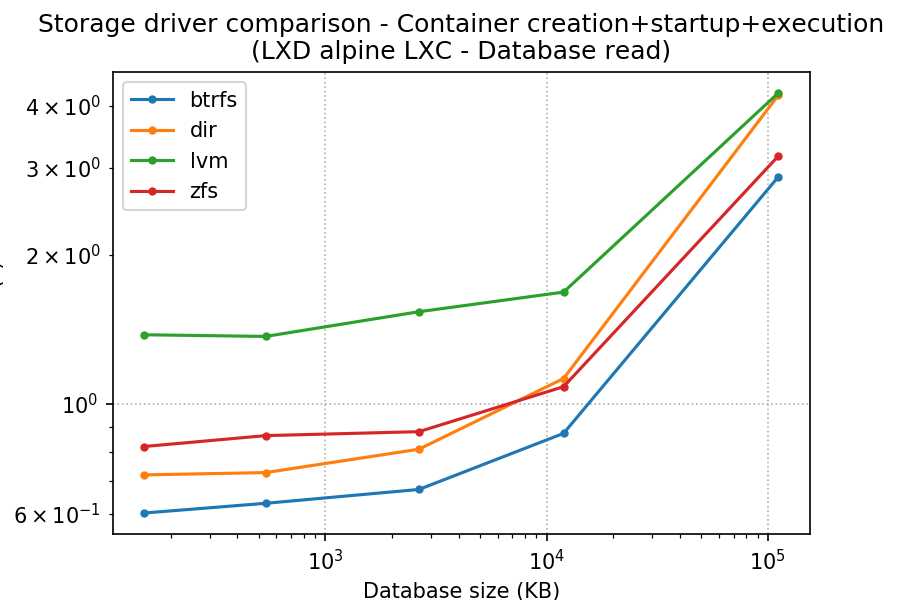
\includegraphics[width=\linewidth]{images/storage-driver/storage-driver-full-LXD-alpine-LXC---Database-read.png}
      \caption{Creation, startup and execution time of containers used for database reading performance test.}
      \label{fig:storage-driver:lxc:db-read-full}
    \end{subfigure}
    \begin{subfigure}{.5\textwidth}
      \centering
      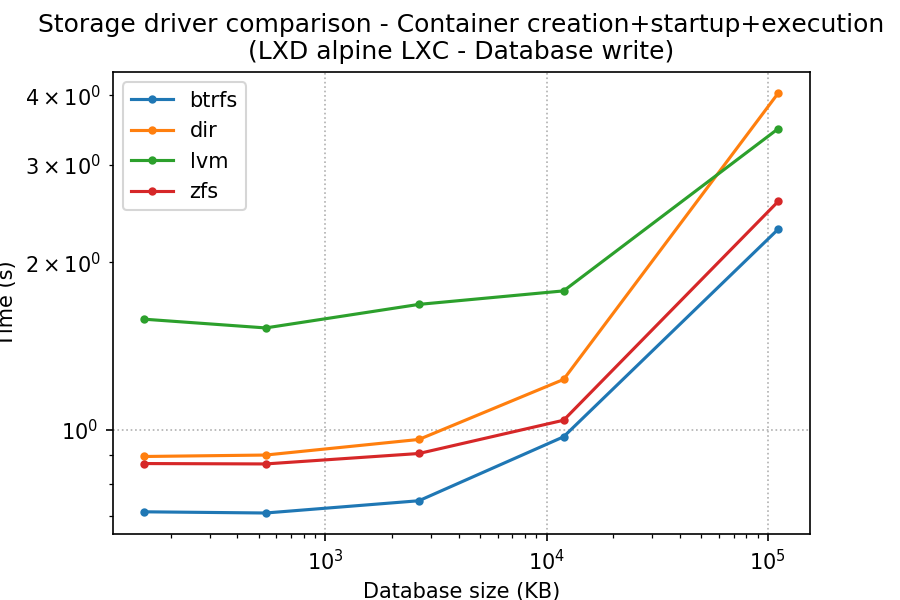
\includegraphics[width=\linewidth]{images/storage-driver/storage-driver-full-LXD-alpine-LXC---Database-write.png}
      \caption{Creation, startup and execution time of containers used for database writing performance test.}
      \label{fig:storage-driver:lxc:db-write-full}
    \end{subfigure}
    
    \caption{Database read and write tests for containers launched with LXD and LXC, based on an Alpine image}
    \label{fig:storage-driver:lxc:db}
\end{figure}

\begin{figure}[!h]
    \begin{subfigure}{.5\textwidth}
      \centering
      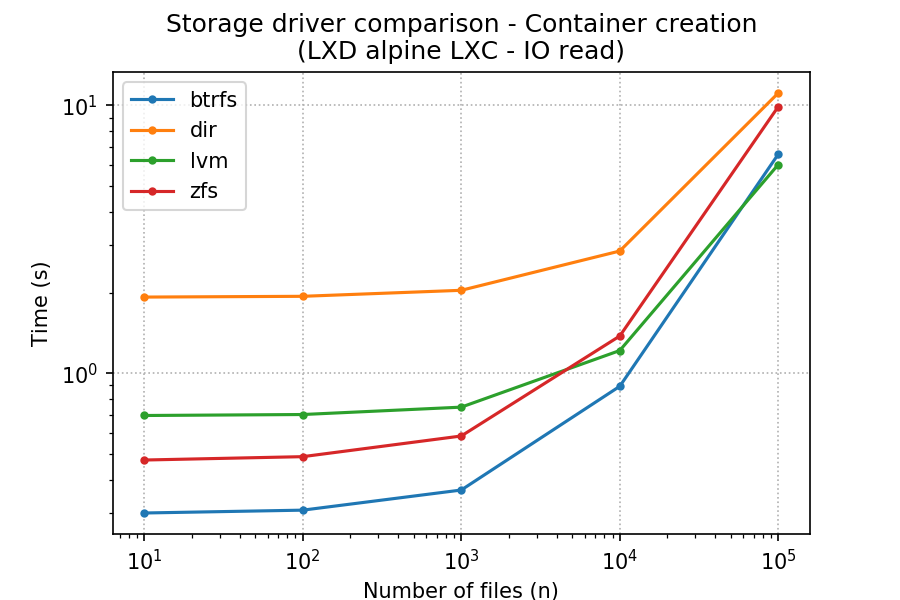
\includegraphics[width=\linewidth]{images/storage-driver/storage-driver-creation-LXD-alpine-LXC---IO-read.png}
      \caption{Average creation time of containers depending on the number of files in one folder.}
      \label{fig:storage-driver:lxc:io-read-create}
    \end{subfigure}
    \begin{subfigure}{.5\textwidth}
      \centering
      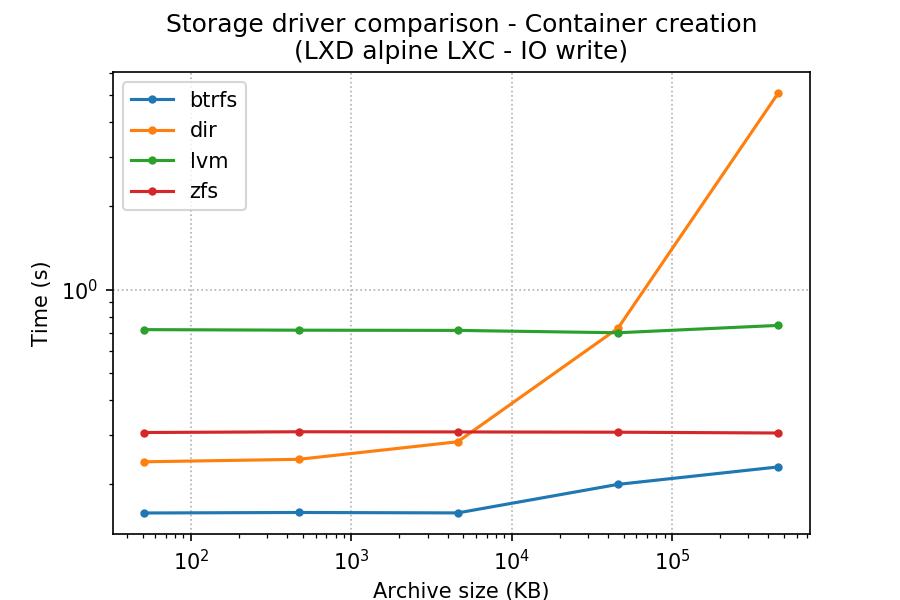
\includegraphics[width=\linewidth]{images/storage-driver/storage-driver-creation-LXD-alpine-LXC---IO-write.png}
      \caption{Average creation time of containers depending on the size of the archive containing all the files.}
      \label{fig:storage-driver:lxc:io-write-create}
    \end{subfigure}
    
    % \begin{subfigure}{.5\textwidth}
    %   \centering
    %   \includegraphics[width=\linewidth]{images/storage-driver/storage-driver-startup-LXD-alpine-LXC---IO-read.png}
    %   \caption{Starting time of containers used for IO reading performance test.}
    %   \label{fig:storage-driver:lxc:io-read-start}
    % \end{subfigure}
    % \begin{subfigure}{.5\textwidth}
    %   \centering
    %   \includegraphics[width=\linewidth]{images/storage-driver/storage-driver-startup-LXD-alpine-LXC---IO-write.png}
    %   \caption{Starting time of containers used for IO writing performance test.}
    %   \label{fig:storage-driver:lxc:io-write-start}
    % \end{subfigure}
    
    \begin{subfigure}{.5\textwidth}
      \centering
      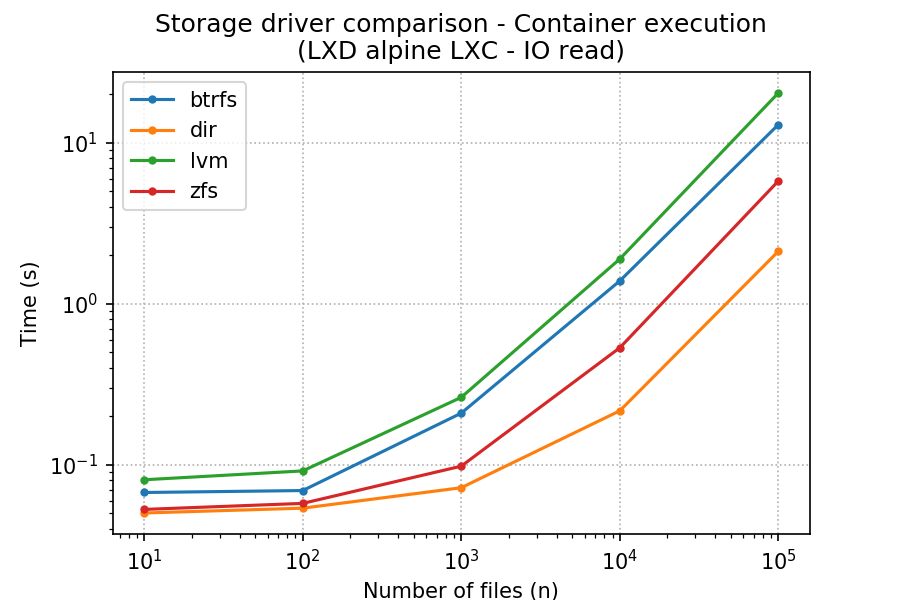
\includegraphics[width=\linewidth]{images/storage-driver/storage-driver-execution-LXD-alpine-LXC---IO-read.png}
      \caption{Average total reading time for n files.}
      \label{fig:storage-driver:lxc:io-read-exec}
    \end{subfigure}
    \begin{subfigure}{.5\textwidth}
      \centering
      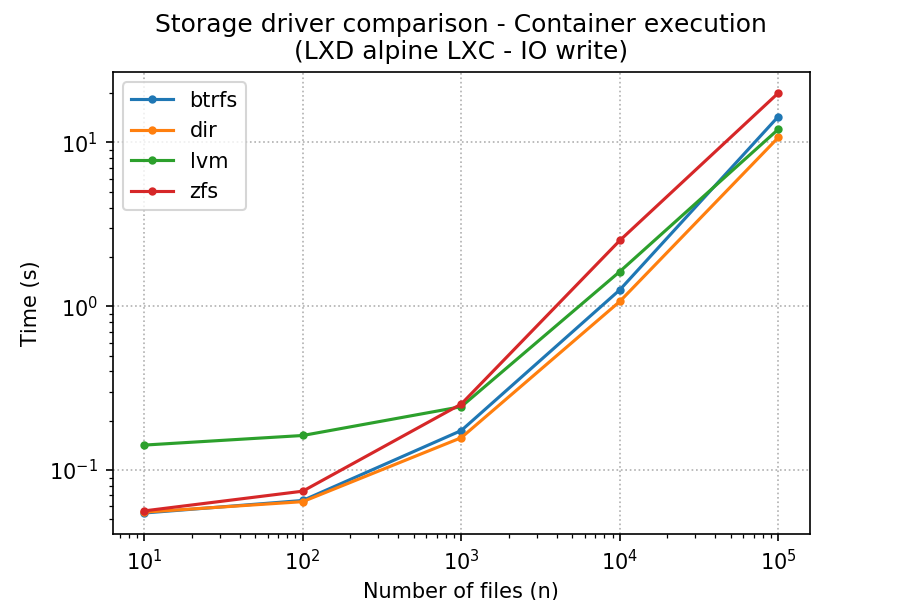
\includegraphics[width=\linewidth]{images/storage-driver/storage-driver-execution-LXD-alpine-LXC---IO-write.png}
      \caption{Average extracting time of n files from one (non-compressed) archive.}
      \label{fig:storage-driver:lxc:io-write-exec}
    \end{subfigure}
    
    \begin{subfigure}{.5\textwidth}
      \centering
      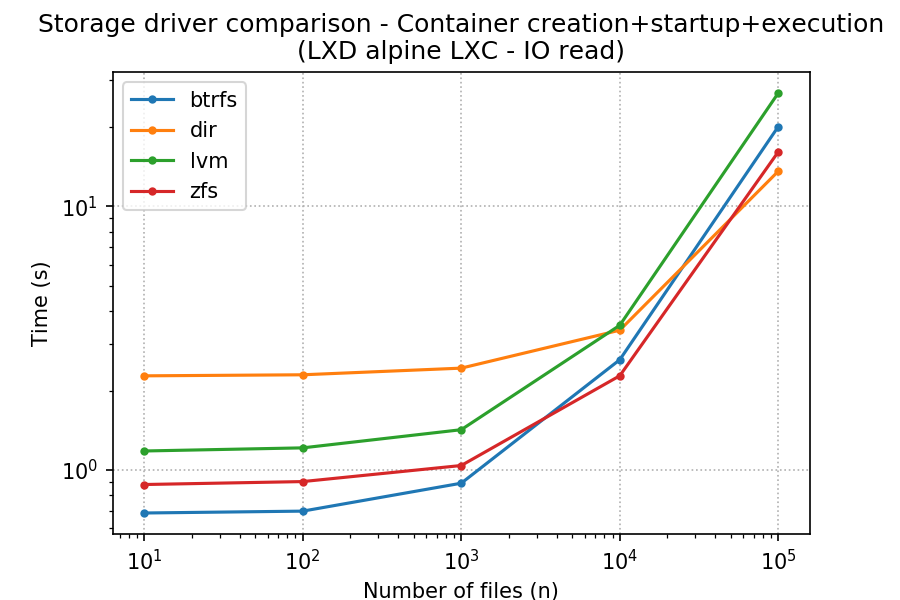
\includegraphics[width=\linewidth]{images/storage-driver/storage-driver-full-LXD-alpine-LXC---IO-read.png}
      \caption{Average creation, startup and execution time of containers used for IO reading performance test.}
      \label{fig:storage-driver:lxc:io-read-full}
    \end{subfigure}
    \begin{subfigure}{.5\textwidth}
      \centering
      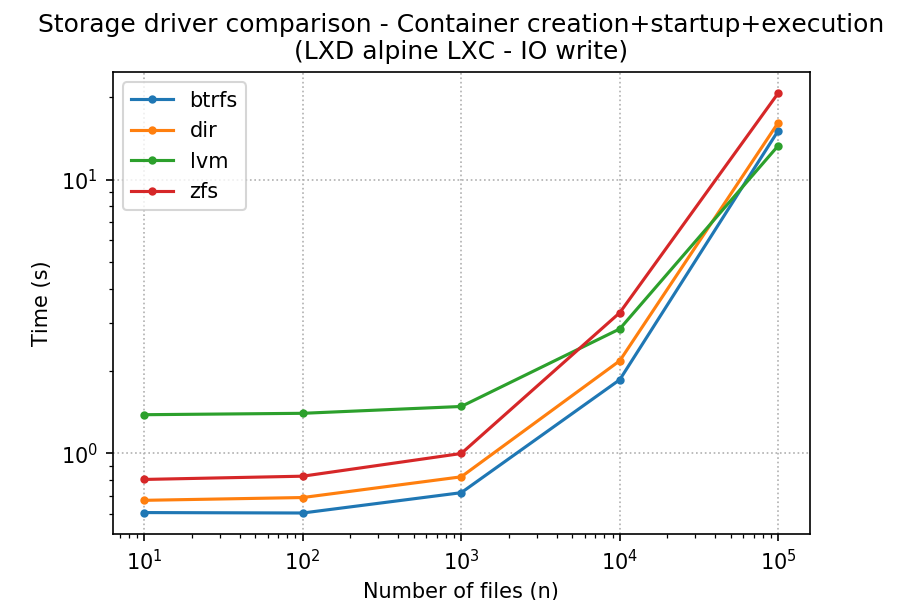
\includegraphics[width=\linewidth]{images/storage-driver/storage-driver-full-LXD-alpine-LXC---IO-write.png}
      \caption{Average creation, startup and execution time of containers used for IO reading performance test.}
      \label{fig:storage-driver:lxc:io-write-full}
    \end{subfigure}
    
    \caption{IO read and write tests for containers launched with Docker and runc, based on an Alpine image}
    \label{fig:storage-driver:lxc:io}
\end{figure}

LXD doesn't propose any file-based copy-on-write solution here.  We have dir, which corresponds to vfs for Docker, its full copy on creation is quite obvious on Figure \ref{fig:storage-driver:lxc:io-write-create}.  On Figure \ref{fig:storage-driver:lxc:io-read-create} though, it seems that all different storage driver suffer from the high amount of files to handle (still less than dir of course).  Overall, from Figure \ref{fig:storage-driver:lxc:db} and \ref{fig:storage-driver:lxc:io}, we can see that btrfs is the driver to go with, even though zfs provide decent execution performance, the cost of creating a container with that file system makes it not worth it to use it (for those tests at least).

\subsection{Container runtime}



\subsection{Container manager}

\subsection{Base image}

\subsection{Rootless container}

\section{Best overal solution}
